\section{Evaluación}

\subsection{Comparativa entre heurísticas de gestión de mapa}

En la Figura \ref{fig:mascaras_original} se muestra un ejemplo de una imagen correspondiente al conjunto de datos empleado para evaluar el trabajo. Podemos observar que hay superficies planas, telas levemente arrugadas y algunas cajas con texturas.

\begin{figure}[H]
    \centering
    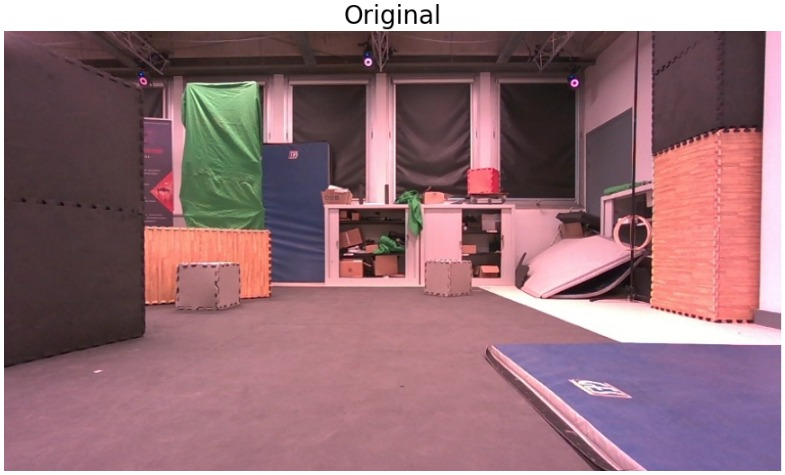
\includegraphics[width=0.7\linewidth]{../imagenes_implementacion/mascaras_original.png}
    \caption{Primera imagen de la secuencia \textit{Line} del conjunto de datos \textit{VIGS-Fusion}.}
    \label{fig:mascaras_original}
\end{figure}

Ahora, en la Figura \ref{fig:masks} se presentan las máscaras obtenidas por cada una de las heurísticas implementadas. Se puede apreciar que la máscara de Fourier genera bordes gruesos y es más sensible a zonas de alta variación de frecuencia, como el fondo de la imagen. Sobel, por su lado, genera bordes gruesos y un poco más sensibles a las texturas, aunque con más precisión para las zonas de alta variación. Laplace, en cambio, es muy sensible al ruido, generando bordes menos definidos. Finalmente, Canny produce bordes delgados y bien definidos, pero con una cobertura mucho menor, especialmente es zonas texturadas, lo que puede resultar en una máscara demasiado escasa para guiar la densificación de gaussianas de manera efectiva.

\begin{figure}[H]
    \centering

    \begin{subfigure}{0.48\textwidth}
        \centering
        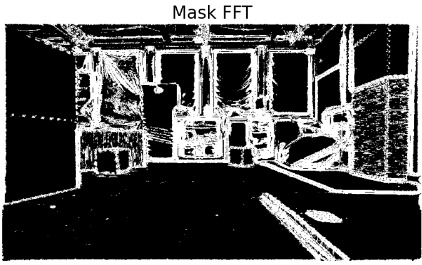
\includegraphics[width=\linewidth]{../imagenes_implementacion/mask_fft.png}
        \caption{FFT}
    \end{subfigure}
    \hfill
    \begin{subfigure}{0.48\textwidth}
        \centering
        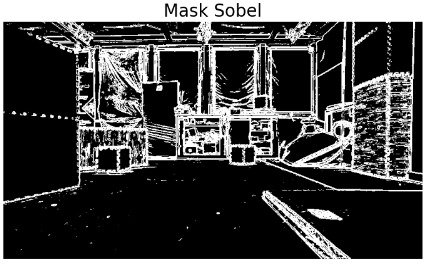
\includegraphics[width=\linewidth]{../imagenes_implementacion/mask_sobel.png}
        \caption{Sobel}
    \end{subfigure}

    \vspace{0.5em}

    \begin{subfigure}{0.48\textwidth}
        \centering
        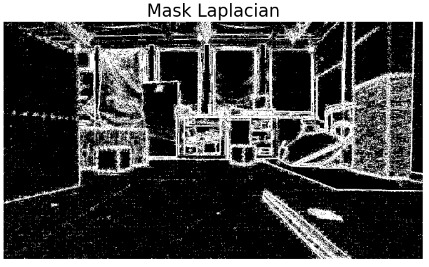
\includegraphics[width=\linewidth]{../imagenes_implementacion/mask_laplace.png}
        \caption{Laplace}
    \end{subfigure}
    \hfill
    \begin{subfigure}{0.48\textwidth}
        \centering
        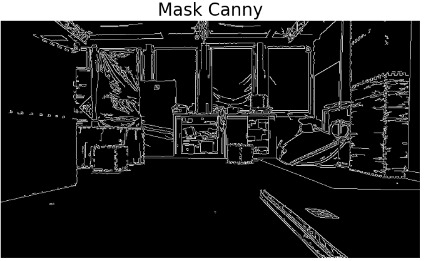
\includegraphics[width=\linewidth]{../imagenes_implementacion/mask_canny.png}
        \caption{Canny}
    \end{subfigure}

    \caption{Comparación de máscaras obtenidas mediante distintos métodos.}
    \label{fig:masks}
\end{figure}

Luego, comparamos las métricas fijando un conjunto de datos.

\begin{table}[H]
\centering
\caption{Comparación de funciones de selección de keyframes sobre la secuencia \textit{Line}.}
\label{tab:line_ablation}
\begin{tabular}{lcccc}
\hline
\textbf{Método} & \textbf{Track/img [ms]} & \textbf{Map/img [ms]} & \textbf{PSNR [dB]} & \textbf{ATE RMSE} \\
\hline
F [VIGS]      & 49.71 & 8.92  & 21.44 & 9.12 \\
F [Fourier]   & 50.23 & 12.09 & 28.13 & 9.54 \\
F [Canny]     & 53.58 & 9.89  & 26.11 & 9.02 \\
F [Sobel]     & 52.02 & 9.21  & 27.81 & 8.87 \\
F [Laplacian] & 52.95 & 11.96 & 27.92 & 8.95 \\
\hline
\end{tabular}
\end{table}

En la tabla \ref{tab:line_ablation} podemos observar que el uso de máscaras de frecuencia mejora la calidad visual sin un costo añadido significativo. En particular, el método basado en Sobel logra un PSNR de 27.31 dB sin tener un impacto costoso en los tiempos, mientras que Fourier logra un PSNR de 28.13 dB, siendo el de mayor calidad, pero con un costo de mapeo más elevado.

Debido a que la gestión de mapa funciona a partir de un muestreo fino en las zonas de alta frecuencia, y uno más espaciado en las de baja, es esperable que los métodos que capturan una mayor región de la imagen logren un mejor PSNR. Sin embargo, debido a que buscamos un método para uso a tiempo real, tomamos el balance entre calidad y costo y empleamos en el resto del trabajo Sobel.

\subsection{Comparativa con VIGS-Fusion}

A continuación, presentamos una comparativa evaluando nuestro nodo y el de VIGS-Fusion utilizando el conjunto de datos mencionado. Para cada secuencia, se evalúan las métricas ejecutando a tiempo real, es decir, perdiendo todos los fotogramas que no llegan a procesarse. Los resultados se resumen en la Tabla \ref{tab:results_comparison}. Las secuencias que poseen ciclos poseen un único ciclo justo al final, y son \textit{Square-Shape} y \textit{Rotation-Only}. Las métricas fueron tomadas con una GPU NVIDIA RTX 3090 y una CPU Intel i5-9400F.


\begin{table}[H]
\centering
\caption{Comparación de métricas entre la configuración propuesta y VIGS-Fusion.}
\label{tab:results_comparison}
\begin{tabular}{llcccc}
\hline
\textbf{Dataset} & \textbf{Método} & \textbf{Track [ms]} & \textbf{Map [ms]} & \textbf{PSNR [dB]} & \textbf{ATE} \\
\hline
                % TRACK % MAP % PSNR % ATE
\multirow{2}{*}{Line}
& Nuestro       & 52.02 & 9.41 & 27.51 & 8.87 \\
& VIGS-Fusion  & 56.35  & 12.32 & 22.19& 9.95 \\
\hline

\multirow{2}{*}{Square-Shape}
& Nuestro       & 57.93 & 15.19 & 24.28 & 16.73 \\
& VIGS-Fusion  & 54.49  & 19.50 & 22.19& 21.52     \\
\hline

\multirow{2}{*}{Rotation-Only}
& Nuestro       & 42.11 & 10.38 & 25.08 & 18.84 \\
& VIGS-Fusion  & 39.91   & 17.11 & 20.31 & 24.95     \\
\hline

\multirow{2}{*}{Line-Rot}
& Nuestro       & 43.73 & 7.67 & 25.77 & 11.16 \\
& VIGS-Fusion  & 48.02  & 9.89 & 18.59  & 11.82      \\
\hline

\end{tabular}
\end{table}

\subsection{Visualización}

A continuación, se presentan algunas visualizaciones de los resultados obtenidos por nuestro método. En aquellas visualizaciones donde se pueda observar el recorrido, se muestra únicamente la posición de los keyframes y submapas, sin mostrar la trayectoria estimada en todo momento. De este modo podemos apreciar los criterios de selección de keyframes y de inicio de submapas. Es importante tener en cuenta que la trayectoria sigue la información de la IMU entre keyframe y keyframe, recibiendo correcciones de la cámara únicamente en los keyframes, por ello es importante que los mismos estén bien distribuidos.

\begin{figure}[H]
    \centering

    \begin{subfigure}{0.49\textwidth}
        \centering
        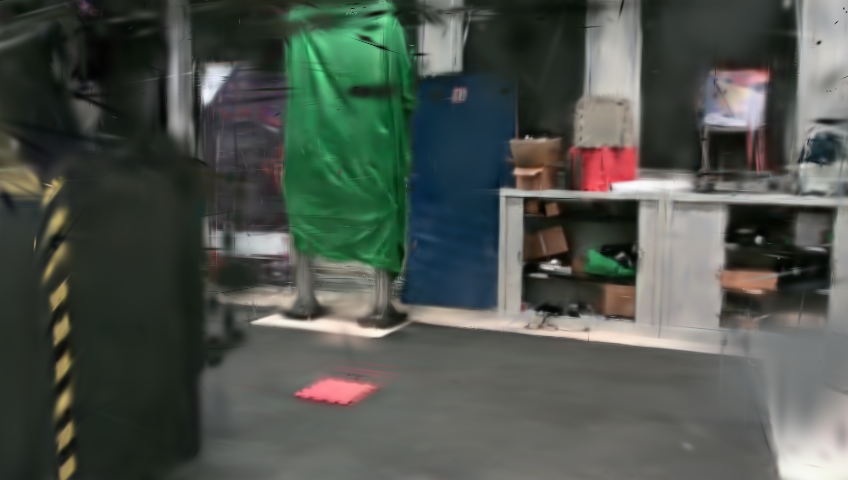
\includegraphics[width=\linewidth]{../imagenes_resultados/ejemplo_1.png}
        \caption{Mapa visto desde el recorrido.}
        \label{fig:ejemplo_izq1}
    \end{subfigure}
    \hfill
    \begin{subfigure}{0.49\textwidth}
        \centering
        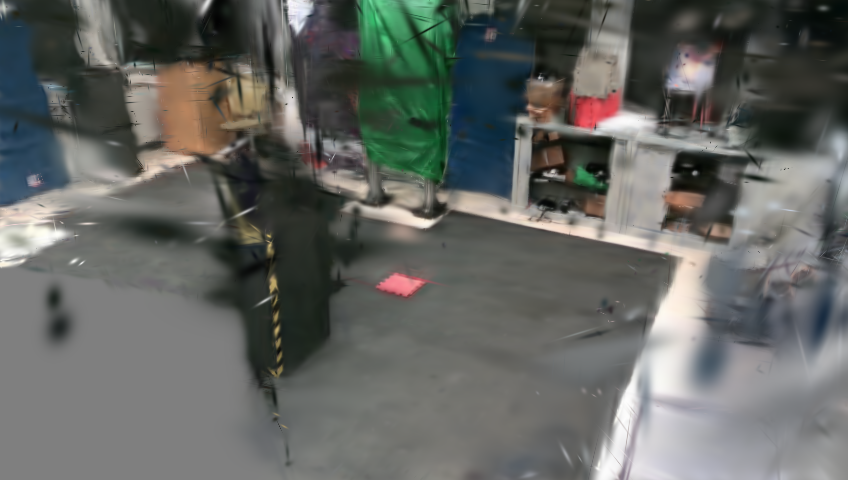
\includegraphics[width=\linewidth]{../imagenes_resultados/ejemplo_3.png}
        \caption{Mapa desde una posición distinta.}
        \label{fig:ejemplo_der1}
    \end{subfigure}

    \caption{Se observa cómo podemos navegar la reconstrucción del mapa más allá de adherirnos al recorrido del robot.}
    \label{fig:comparacion1}
\end{figure}

\begin{figure}[H]
    \centering

    \begin{subfigure}{0.49\textwidth}
        \centering
        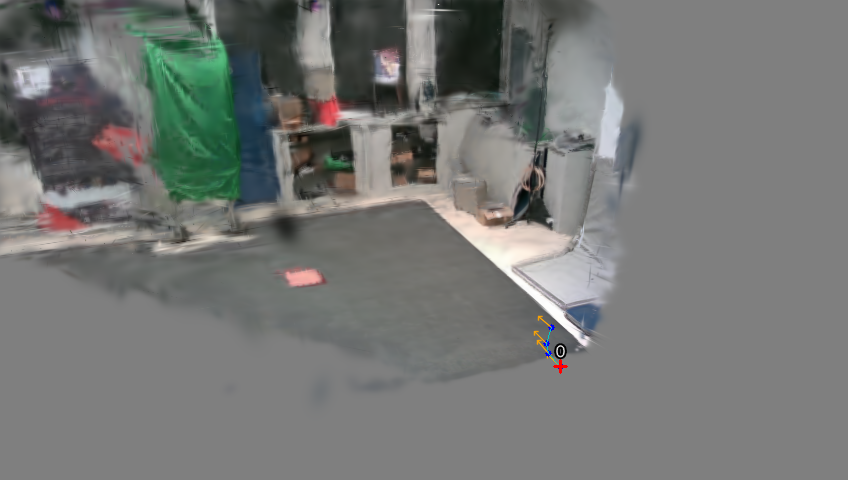
\includegraphics[width=\linewidth]{../imagenes_resultados/ejemplo2_1.png}
        \caption{Inicio del mapa.}
        \label{fig:ejemplo_izq2}
    \end{subfigure}
    \hfill
    \begin{subfigure}{0.49\textwidth}
        \centering
        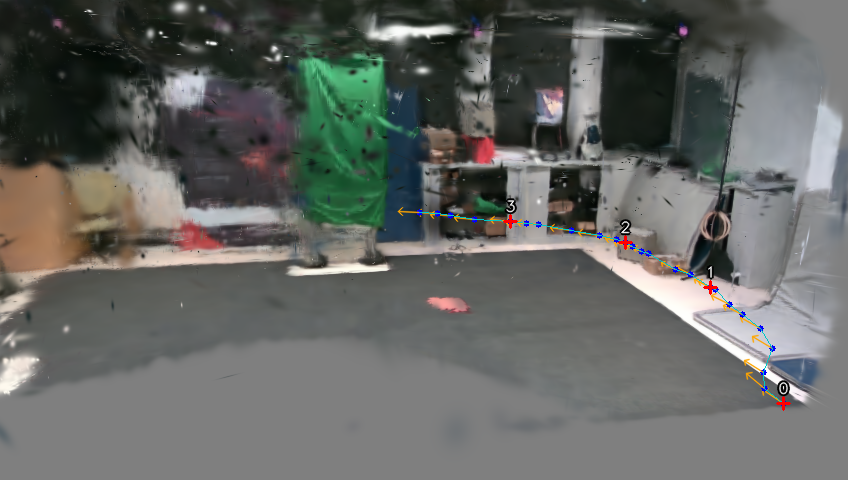
\includegraphics[width=\linewidth]{../imagenes_resultados/ejemplo2_2.png}
        \caption{Continuación del mapa.}
        \label{fig:ejemplo_der2}
    \end{subfigure}

    \caption{Cada cruz roja numerada es el inicio de un submapa, donde cada punto azul es un keyframe del mismo. Se observa cómo el mapa se va reconstruyendo a medida que el robot avanza.}
    \label{fig:comparacion2}
\end{figure}

\begin{figure}[H]
    \centering

    \begin{subfigure}{0.49\textwidth}
        \centering
        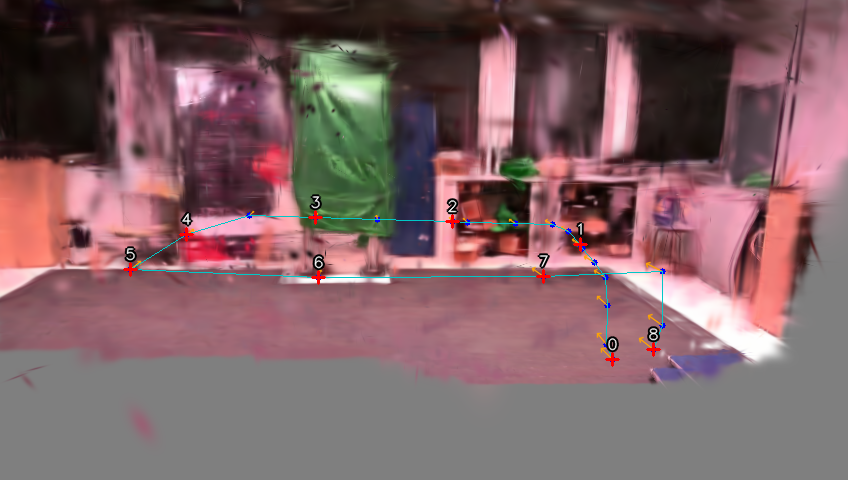
\includegraphics[width=\linewidth]{../imagenes_resultados/ejemplo3_1.png}
        \caption{Mapa sin cierre de ciclos.}
        \label{fig:ejemplo_izq3}
    \end{subfigure}
    \hfill
    \begin{subfigure}{0.49\textwidth}
        \centering
        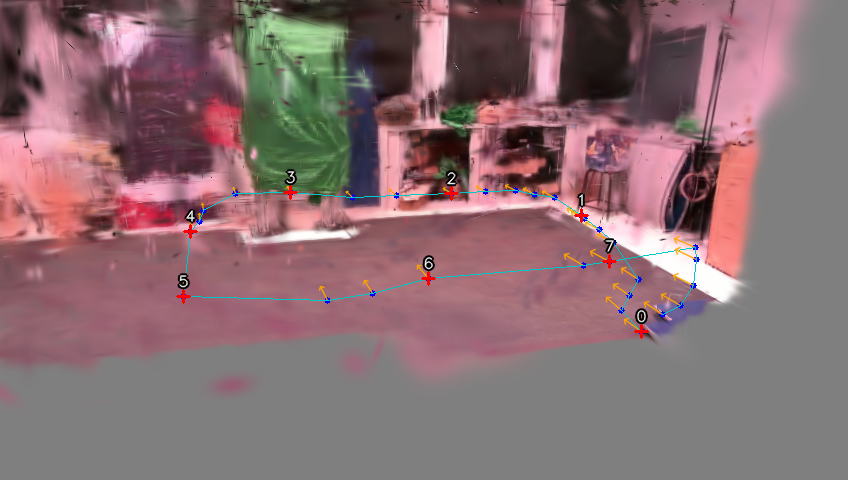
\includegraphics[width=\linewidth]{../imagenes_resultados/ejemplo3_2.png}
        \caption{Mapa con cierre de ciclos.}
        \label{fig:ejemplo_der3}
    \end{subfigure}

    \caption{La secuencia \textit{Square-Shape} posee un ciclo al final del recorrido. En la imagen de la izquierda se observa el mapa sin aplicar cierre de ciclos, donde se puede apreciar una desviación acumulada que genera una discontinuidad en el mapa. En la imagen de la derecha, al aplicar cierre de ciclos, se corrige esta desviación y se obtiene un recorrido consistente.}
    \label{fig:comparacion3}
\end{figure}